% !TEX root = ./main.tex
\graphicspath{{figures_squarecylinder/}}% Set graphics path location

\subsection{LES of Flow Over a Square Cylinder at Re = 21,400}\label{sqcyl}

Using the FR method to recover the fourth-order accurate SD scheme, the flow over a square cylinder of side $D$ in a domain of $21D \times 12D \times 3.2D$ (see Figure \ref{sqcylmesh}) at $Re = 21,400$ and Mach 0.3 was simulated, for which Laser Doppler Velocimetry (LDV) experimental data is available~\cite{lyn1994,lyn1995}.
A tetrahedral mesh of 87,178 elements was generated giving a total of 1.74M degrees of freedom (D0F) since there are 20 solution points per element at fourth order accuracy.
Time discretization was by the fourth-order five-stage explicit RK scheme.
A total time of 250 seconds was simulated and time-averaged quantities were calculated over the last 100 seconds (approx. 5 flow-through periods).
The WSM model (see Section \ref{lesmodels}) based on the modal Vandermonde filter~\cite{bull2014a} was used with the Breuer-Rodi three-layer wall model~\cite{breuer1994} within 0.2D of the wall.
The computation took around 60 hours on 7 GPUs in the lab's own cluster.
Figure \ref{sqcylmesh} shows the computational mesh including all the DoFs.
Figure \ref{sqcylqcrit} shows an isosurface of the $q$-criterion colored by velocity magnitude, illustrating the structures present in the turbulent boundary layer and wake.
Figures \ref{sqcylplots} (a, b) show the normalized mean streamwise and vertical velocity components $\langle u \rangle/u_B$ and $\langle v \rangle/u_B$ respectively along several vertical lines in the wake.
Figures \ref{sqcylplots} (c, d) show the normalized mean Reynolds stress components $\langle u'u' \rangle/u_B^2$ and $\langle u'v' \rangle/u_B^2$ along the same lines.
For comparison, high-order LES results computed by Lodato and Jameson~\cite{lodato2012b} using the SD method and the WSM model on a hexahedral mesh of 2.3M DoF are plotted.
Mean velocities are accurately predicted although the accuracy is reduced near the cylinder owing to the coarse tetrahedral resolution in the boundary layer.
The Reynolds stresses are less accurately predicted than the mean velocities but are broadly correct.
These results highlight the advantages of using HiFiLES for LES of turbulent flows: the ability to obtain good results on coarse meshes and the ability to use unstructured tetrahedral meshes.


\begin{figure}[h] \tt
\centering
\subfigure[geometry]{
\includegraphics*[width=0.61\textwidth]{sqcyl-geom-small}}
\subfigure[boundary layer mesh]{
\includegraphics*[width=0.35\textwidth]{sqcyl-tet-coarse3-blmesh}}
\caption{Square cylinder geometry and tetrahedral boundary layer mesh showing all degrees of freedom}
\label{sqcylmesh}
\end{figure}

\begin{figure}[h] \tt
\centering
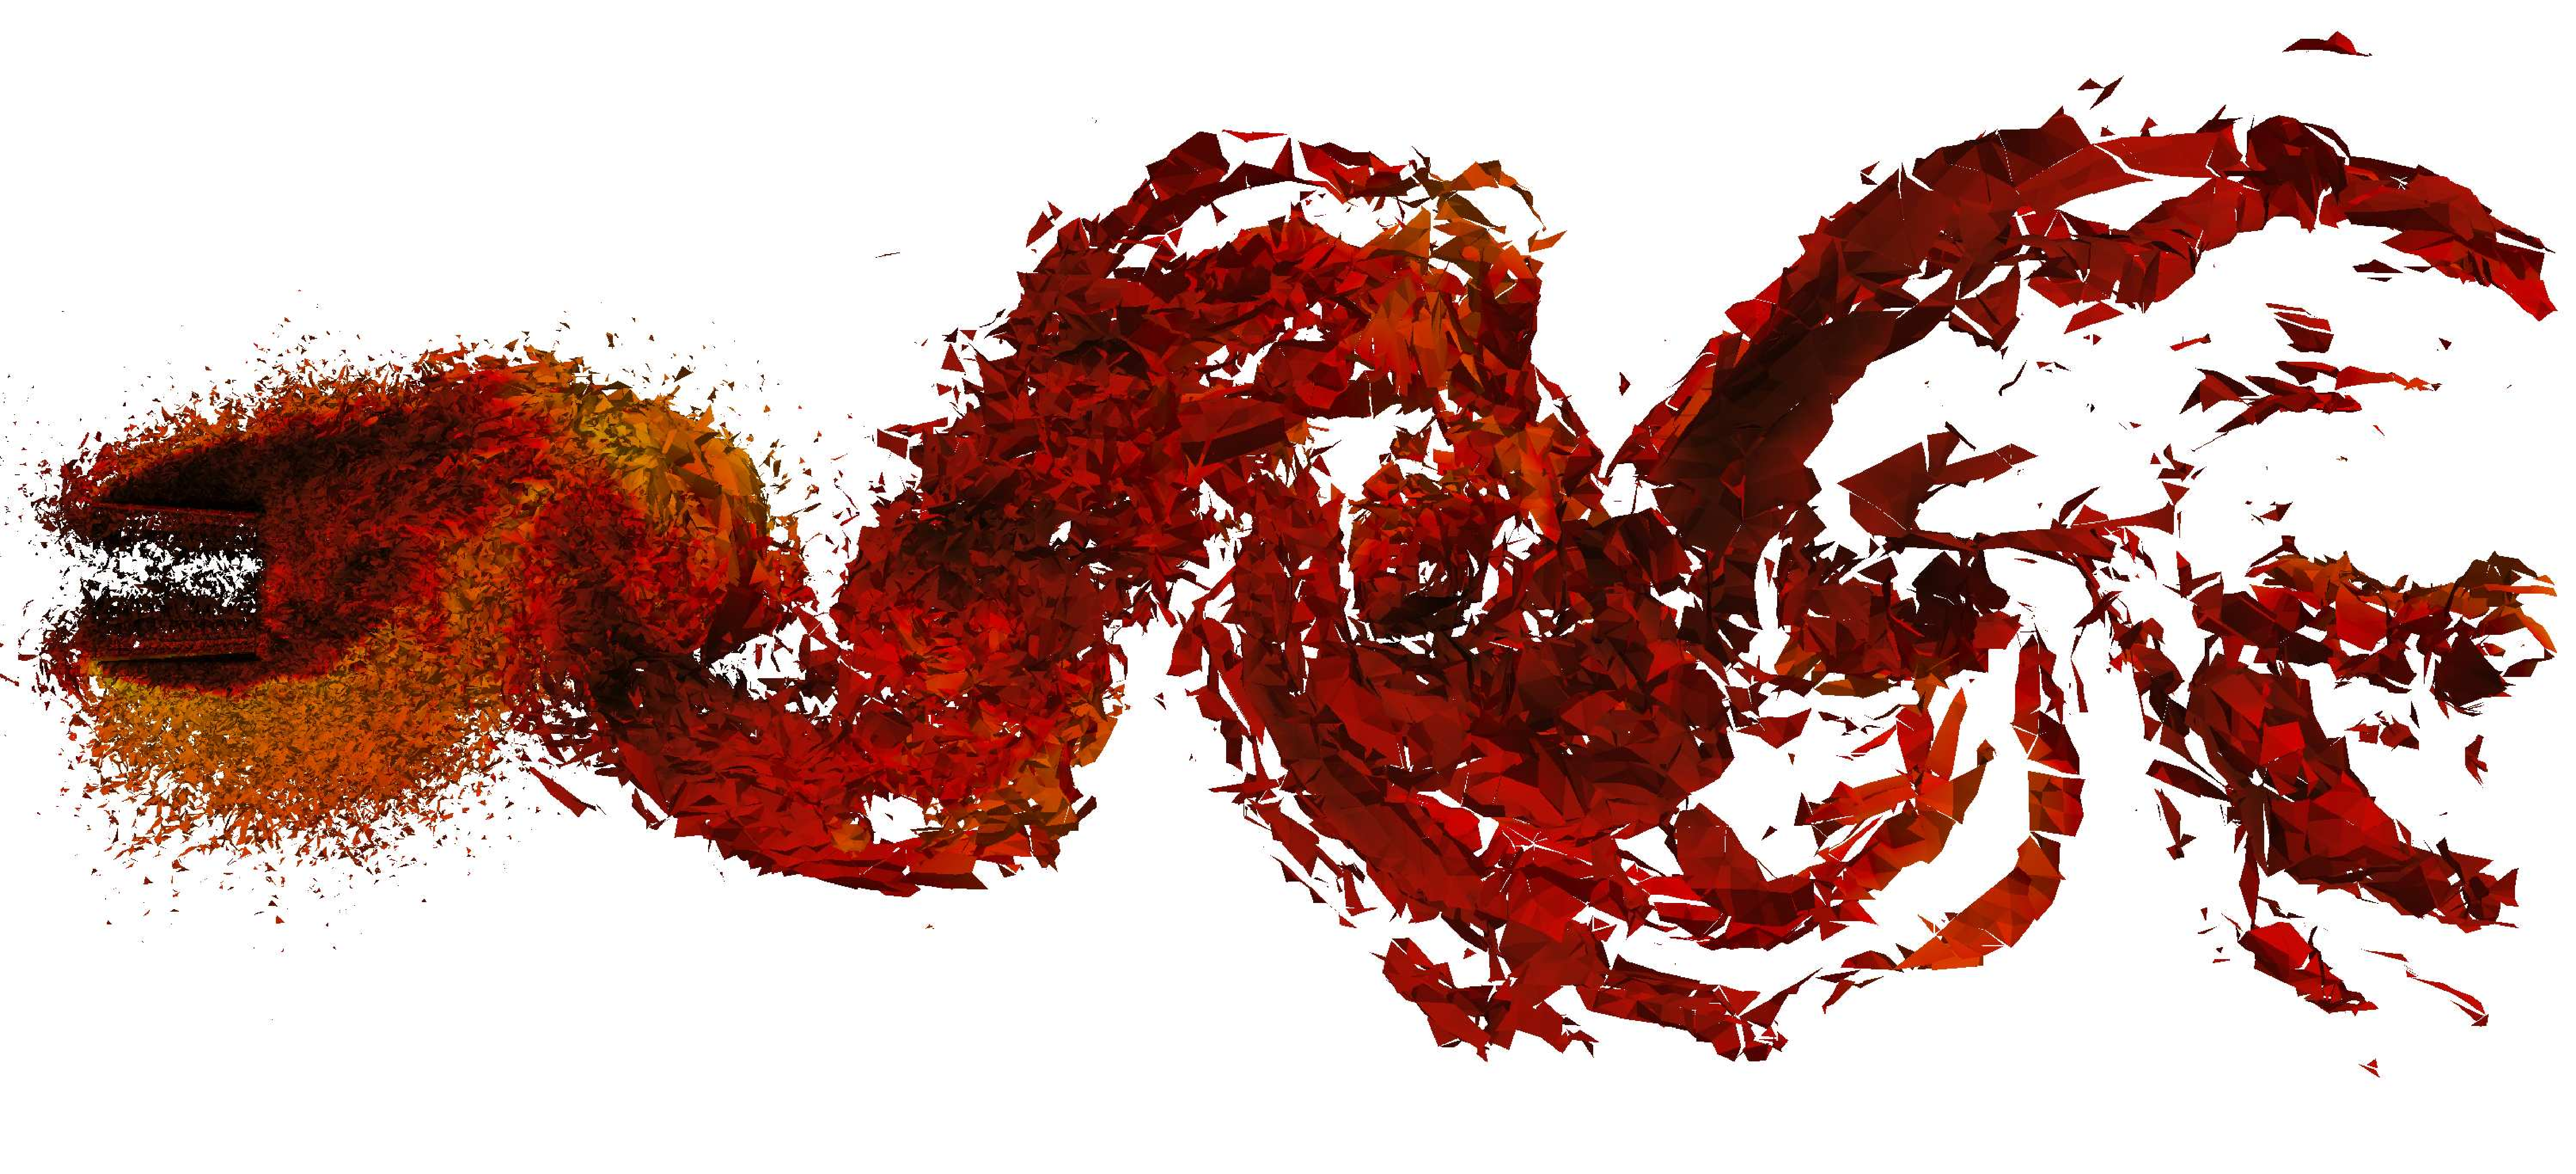
\includegraphics[width=0.9\textwidth]{sqcyl-tet-wsm-newwallfn-coarse3-qcrit-010-velomag.pdf}
\caption{Isosurface of the $q$-criterion colored by velocity magnitude showing the wake behind the square cylinder}
\label{sqcylqcrit}
\end{figure}

\begin{figure}[h]
\centering
\subfigure[Mean streamwise velocity $\langle u \rangle/u_B$]{
\includegraphics*[width=0.8\textwidth]{sqcyl-tet-wsm-newfilt-coarse-fixbc-meanu-vprofile-small.pdf}}\\
\subfigure[Mean vertical velocity $\langle v \rangle/u_B$]{
\includegraphics*[width=0.8\textwidth]{sqcyl-tet-wsm-newfilt-coarse-fixbc-meanv-vprofile-small.pdf}}\\
\subfigure[Mean Reynolds stress $\langle u'u' \rangle/u_B^2$]{
\includegraphics*[width=0.8\textwidth]{sqcyl-tet-wsm-newfilt-coarse-fixbc-meanuu-vprofile-small.pdf}}\\
\subfigure[Mean Reynolds stress $\langle u'v' \rangle/u_B^2$]{
\includegraphics*[width=0.8\textwidth]{sqcyl-tet-wsm-newfilt-coarse-fixbc-meanuv-vprofile-small.pdf}}
\caption{\small (a) Mean streamwise and vertical velocity and mean Reynolds stresses along vertical lines in the wake.
(---) current results, (- - - ) 4th order SD+WSM on hexahedral mesh by Lodato and Jameson~\cite{lodato2012b}, ($\circ$) LDV experiments by Lyn et al.~\cite{lyn1994,lyn1995}.}
\label{sqcylplots}
\end{figure}

